\documentclass[a4paper,12pt,dvipdfmx]{exam}
\usepackage{graphicx}
\usepackage{amssymb}
\usepackage{caption}
\usepackage{subcaption}
\usepackage{multirow}
\usepackage{siunitx}

\firstpageheader{EE5907}{CA2}{\today}
\runningheader{EE5907}{CA2 (Continued)}{\today}
\footer{}{\thepage}{}

\graphicspath{ {figures/} }

\sisetup{round-mode = places,
scientific-notation = fixed}

\begin{document}
\begin{questions}
    \question PCA based data distribution visualizations

    Let the data matrix $\mathbf{X}$ be of $n \times p$ size.\\
    First, perform SVD:
    \begin{equation}
        \mathbf{X}=\mathbf{USV^\intercal}
    \end{equation}
    The columns of $\mathbf{US}$ are the principal components and the columns of $\mathbf{V}$ are the eigenfaces.\\
    For the principal components, only calculation for the highest dimension is necessary. For reduction to
    dimension $k$, the first $k$ principal components can be obtained from the first $k$ columns of
    $\mathbf{U}$ and the diagonal matrix formed by the first $k$ values along the diagonal of $\mathbf{S}$.

    \begin{figure}[h]
        \centering
        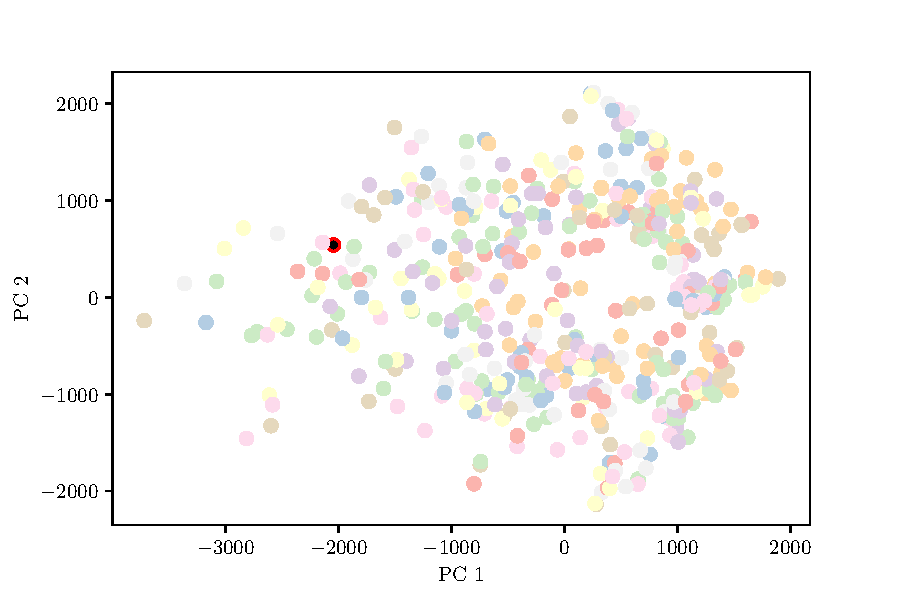
\includegraphics[width=0.75\textwidth]{pca_2d}
        \caption{PCA projected data vector in 2D.}
        \label{fig:pca_2d}
    \end{figure}

    \begin{figure}[ht]
        \centering
        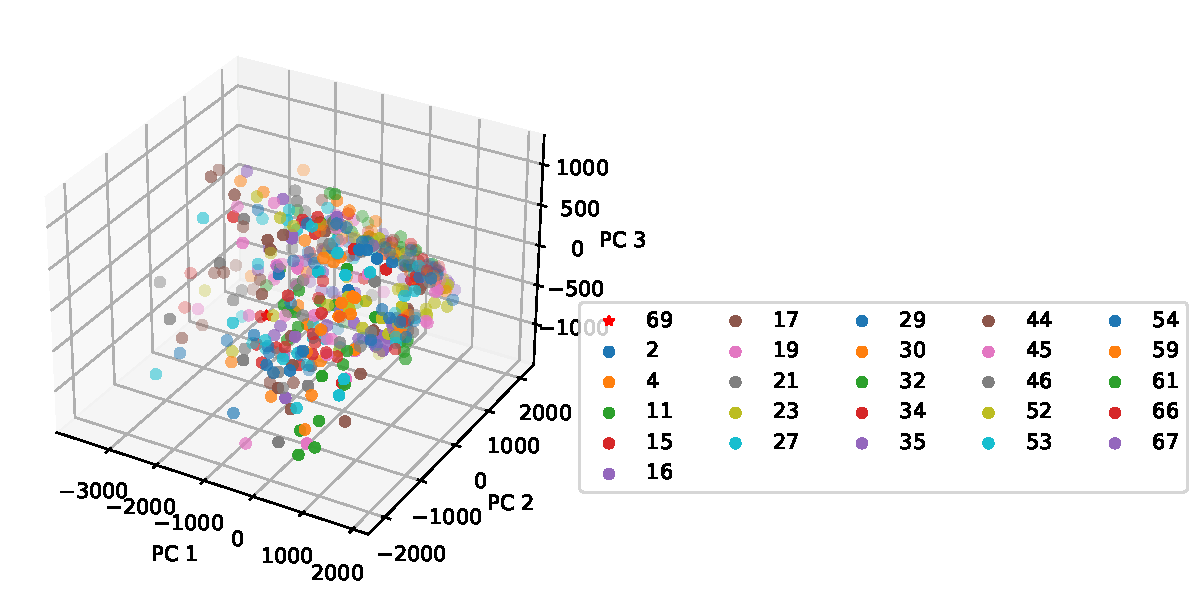
\includegraphics[width=0.75\textwidth]{pca_3d}
        \caption{PCA projected data vector in 3D.}
        \label{fig:pca_3d}
    \end{figure}

    \begin{figure}[ht]
        \centering
        \begin{subfigure}[b]{0.3\textwidth}
            \centering
            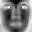
\includegraphics[width=\textwidth]{eigenface0}
            \caption{eigenface 0}
            \label{fig:eigenface0}
        \end{subfigure}
        \hfill
        \begin{subfigure}[b]{0.3\textwidth}
            \centering
            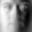
\includegraphics[width=\textwidth]{eigenface1}
            \caption{eigenface 1}
            \label{fig:eigenface1}
        \end{subfigure}
        \hfill
        \begin{subfigure}[b]{0.3\textwidth}
            \centering
            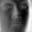
\includegraphics[width=\textwidth]{eigenface2}
            \caption{eigenface 2}
            \label{fig:eigenface2}
        \end{subfigure}
        \caption{Corresponding 3 eigenfaces used for PCA dimensionality reduction.}
        \label{fig:eigenface}
    \end{figure}

    \question PCA plus nearest neighbor classification results

    For classification with PCA, obtain $\mathbf{XV}$, projection of the faces in the test data matrix $\mathbf{X}$ on the
    eigenface space. Each column of $\mathbf{V}$ and therefore each column of $\mathbf{XV}$ corresponds to a principal component.\\
    Again, only calculation for the highest dimension is necessary. The first $k$ projections can be obtained
    with the test data matrix and the first $k$ columns of $\mathbf{V}$.

    It is expected that classfication of selfies is unsuccessful. There are only three selfies in the test
    set and random sampling of 500 images for training included only one selfie which is an outlier in 3D as can be seen from the scatter plots.
    Moreover, my setup and lighting condition differs from those of the images in the PIE data set.

    \begin{center}
        \begin{tabular}{ |c|c|c|c| }
            \hline
            Test Images                & Dimensionality & Accuracy                             \\
            \hline
            \multirow{3}{4em}{CMU PIE} & 40             & \SI{0.49019607843137253e2}{\percent} \\
                                       & 80             & \SI{0.5247058823529411e2}{\percent}  \\
                                       & 200            & \SI{0.552156862745098e2}{\percent}   \\
            \hline
            \multirow{3}{4em}{Selfies} & 40             & \SI{0.0}{\percent}                   \\
                                       & 80             & \SI{0.0}{\percent}                   \\
                                       & 200            & \SI{0.0}{\percent}                   \\
            \hline
        \end{tabular}
    \end{center}

    \question LDA based data distribution visualization
    \question LDA plus nearest neighbor classification results
    \question SVM classification results with different parameter values
    \question CNN classification results with different network architectures
\end{questions}

\end{document}
